\documentclass{report}[pt12]
\usepackage{amsmath}
\usepackage{tikz}
\usepackage[section]{placeins}
\usetikzlibrary{automata, arrows.meta, positioning}



\setcounter{chapter}{+1}

\title{Language and Automata, Assignment 1}
\author{Krzysztof Rudnicki\\ Student number: 307585}
\date{\today}


\begin{document}
\maketitle

	\section{Regular expression}
We are given following regular expression:
\[ a^* + ba^*b + bba^*\]


	\section{Examples of accepted strings}
\begin{enumerate}
\item $ \varepsilon $
\item a
\item bab
\item bba
\item bb
\end{enumerate}


	\input{sections/03-building-nfa-using-thompson-construction-algorithm}
	\section{Transforming NFA into DFA using subset algorithm}
I will use $\epsilon_{cl}$ instead of $\epsilon$-closure for brevity sake.
Final state - $\underline{q_{19}}$ was marked with an $\underline{underline}$ and so did all the states of DFA that contain it.
\[ A = \epsilon_{cl}(q_0) = (q_0, q_1, q_3, q_4, q_6, q_{12}, q_{18}, \underline{q_{19}}) = \underline{A} \]
\[ \epsilon_{cl}(move(\underline{A}, a)) = (\epsilon_{cl}(move(q_0, q_1, q_3, q_4, q_6, q_{12}, q_{18}, \underline{q_{19}}, a))) = \epsilon_{cl}(q_9) = (q_6, q_9, q_{12}, q_{18}, \underline{q_{19}}) = \underline{B}  \]
\[ A = \epsilon_{cl}(move(\underline{A}, b)) = \epsilon_{cl}(move(q_0, q_1, q_3, q_4, q_6, q_{12}, q_{18}, \underline{q_{19}}, b))) = \epsilon_{cl}(q_2, q_7) = (q_2, q_7, q_{10}, q_{15}) = C \]
\[ \epsilon_{cl}(move(\underline{B}, a)) = \epsilon_{cl}(move(q_6, q_9, q_{12}, q_{18}, \underline{q_{19}}), a) = \epsilon_{cl}(q_9) = (q_6, q_9, q_{12}, q_{18}, \underline{q_{19}}) = \underline{B} \]
\[ \epsilon_{cl}(move(\underline{B}, b)) = \epsilon_{cl}(move(q_6, q_9, q_{12}, q_{18}, \underline{q_{19}}), b) = \emptyset \]
\[ \epsilon_{cl}(move(C, a)) = \epsilon_{cl}(move(q_2, q_7, q_{10}, q_{15}), a) = \epsilon_{cl}(q_{13}) = (q_{10}, q_{13}, q_{15}) = D \]
\[ \epsilon_{cl}(move(C, b)) = \epsilon_{cl}(move((q_2, q_7, q_{10}, q_{15}), b) = \epsilon_{cl}(q_{17}) = (q_{17}, q_{18}, \underline{q_{19}}) = \underline{E}  \]
\[ \epsilon_{cl}(move(D, a)) = \epsilon_{cl}(move((q_{10}, q_{13}, q_{15}), a) = \epsilon_{cl}(q_{13}) = (q_{10}, q_{13}, q_{15}) = D  \]
\[ \epsilon_{cl}(move(D, b)) = \epsilon_{cl}(move(q_{10}, q_{13}, q_{15}, b) = \epsilon_{cl}(q_{17}) = (q_{17}, q_{18}, \underline{q_{19}}) = \underline{E} \]
\[ \epsilon_{cl}(move(\underline{E}, a)) = \epsilon_{cl}(move(q_{17}, q_{18}, \underline{q_{19}}), a) = \epsilon_{cl}(\emptyset) = \emptyset \]
\[ \epsilon_{cl}(move(\underline{E}, b)) = \epsilon_{cl}(move(q_{17}, q_{18}, \underline{q_{19}}), b) = \epsilon_{cl}(\emptyset) = \emptyset \]

\subsection{State table}
\begin{center}
\begin{tabular}{||c c c||}
 \hline
 State & a & b \\
 \hline
$\underline{A}$ & $\underline{B}$ & C\\
 \hline
 $\underline{B}$ & $\underline{B}$  & $\emptyset$ \\
 \hline
 C & D & $\underline{E}$\\
 \hline
 D & D & $\underline{E}$\\
 \hline
 $\underline{E}$ & $\emptyset$ & $\emptyset$\\
 \hline
$\emptyset$ & $\emptyset$ & $\emptyset$\\
 \hline
\end{tabular}
\end{center}

\begin{figure}[!htb]
\centering
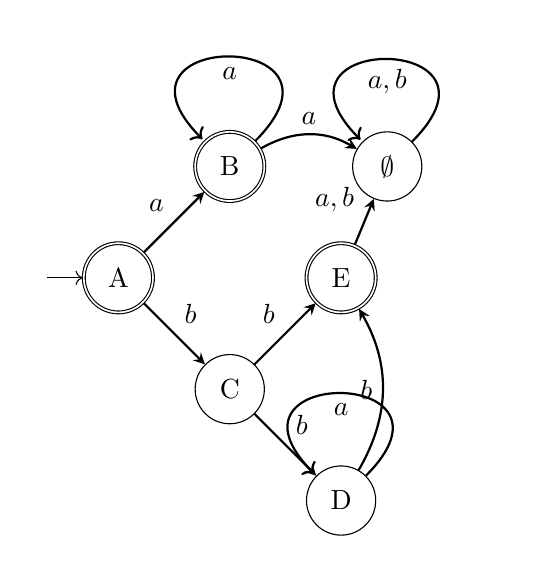
\begin{tikzpicture} [node distance = 2cm, on grid, auto]

  \node (q0) [state, accepting, initial, initial text = {}] {A};
  \node (q1) [state, accepting, above right = of q0] {B};
  \node (q2) [state, below right = of q0] {C};
  \node (q3) [state, accepting, above right = of q2] {E};
  \node (q4) [state, below right = of q2] {D};
  \node (q5) [state, right = of q1] {$\emptyset$};

  \path [-stealth, thick]
  (q0) edge node {$a$}   (q1);

  \path [-stealth, thick]
  (q0) edge node {$b$}   (q2);

  \path [-stealth, thick]
  (q1) edge [loop] node {$a$}   (q1);

  \path [-stealth, thick]
  (q2) edge node {$b$}   (q4);

  \path [-stealth, thick]
  (q2) edge node {$b$}   (q3);

  \path [-stealth, thick]
  (q4) edge [bend right] node {$b$}   (q3);

  \path [-stealth, thick]
  (q4) edge [loop] node {$a$}   (q4);

  \path [-stealth, thick]
  (q1) edge [bend left] node {$a$}   (q5);

  \path [-stealth, thick]
  (q3) edge node {$a, b$}   (q5);

  \path [-stealth, thick]
  (q5) edge [loop] node {$a, b$}   (q5);




\end{tikzpicture}
\caption{DFA graph before minimalization} \label{dfaNominimalization}
\end{figure}


	\section{Constructing minimal state DFA}

\begin{tabular}{|*{7}{c|}}
                               \cline{1-1}
  $\underline{A}$                     \\ \cline{1-2}
  $\underline{B}$ & $x_1$                 \\ \cline{1-3}
  C & $x_1$ & $x_1$           \\ \cline{1-4}
  D & $x_1$ & $x_1$ & $x_2$         \\ \cline{1-5}
  $\underline{E}$ & $x_1$ & $x_1$ & $x_1$ & $x_1$    \\ \cline{1-6}
  $\emptyset$ & $x_1$ & $x_1$ & $x_2$ & $x_2$ & $x_1$ \\ \hline
    & $\underline{A}$ & $\underline{B}$ & C & D & $\underline{E}$ & $\emptyset$ \\ \hline
\end{tabular}

\begin{enumerate}
  \item First I marked (with $x_1$) all the pairs in which at least one of them were final state:
  \[ ([\underline{A}, \emptyset], [\underline{A}, \underline{E}], [\underline{A}, D], [\underline{A}, C], [\underline{A}, \underline{B}]) \]
    \[ ([\underline{B}, \emptyset], ([\underline{B}, \underline{E}], ([\underline{B}, D], ([\underline{B}, C]) \]
    \[ ([\underline{E}, \emptyset], [\underline{E}, C], [\underline{E}, D])\]

  \item We are left with the pairs:
  \[ ([\emptyset , C], [\emptyset , D], [D , C] ) \]
  For pair: $ [\emptyset , C] $ C goes to final state $\underline{E}$ on transition 'b' therefore we mark it with $x_2$
  For pair: $ [\emptyset , D] $ D goes to final state $\underline{E}$ on transition 'b' therefore we mark it with $x_2$
  For pair: $ [D , C] $ both C and D go to final state $\underline{E}$ on transition 'b' therefore we mark it with $x_2$
\end{enumerate}

No states could be minimized! Therefore our final minimal state DFA looks like this:

\begin{figure}[!htb]
\centering
\begin{tikzpicture} [node distance = 2cm, on grid, auto]

\node (q0) [state, accepting, initial, initial text = {}] {A};
\node (q1) [state, accepting, above right = of q0] {B};
\node (q2) [state, below right = of q0] {C};
\node (q3) [state, accepting, above right = of q2] {E};
\node (q4) [state, below right = of q2] {D};
\node (q5) [state, right = of q1] {$\emptyset$};

\path [-stealth, thick]
(q0) edge node {$a$}   (q1);

\path [-stealth, thick]
(q0) edge node {$b$}   (q2);

\path [-stealth, thick]
(q1) edge [loop] node {$a$}   (q1);

\path [-stealth, thick]
(q2) edge node {$a$}   (q4);

\path [-stealth, thick]
(q2) edge node {$b$}   (q3);

\path [-stealth, thick]
(q4) edge node {$b$}   (q3);

\path [-stealth, thick]
(q1) edge [bend left] node {$a, b$}   (q5);

\path [-stealth, thick]
(q3) edge [below loop] node {$a$}   (q3);

\path [-stealth, thick]
(q3) edge node {$a$}   (q5);

\path [-stealth, thick]
(q4) edge [bend right] node {$a$}   (q5);

\path [-stealth, thick]
(q5) edge [loop] node {$a, b$}   (q5);





\end{tikzpicture}
\caption{DFA graph after minimalization} \label{dfaMinimalization}
\end{figure}





\end{document}
